
%(BEGIN_QUESTION)
% Copyright 2008, Tony R. Kuphaldt, released under the Creative Commons Attribution License (v 1.0)
% This means you may do almost anything with this work of mine, so long as you give me proper credit

Calculate the sine of angle $A$ and the tangent of angle $B$ in this triangle:

$$\includegraphics[width=15.5cm]{i03159x01.eps}$$

\vfil 

\underbar{file i03159}
\eject
%(END_QUESTION)





%(BEGIN_ANSWER)

This is a graded question -- no answers or hints given!
 
%(END_ANSWER)





%(BEGIN_NOTES)

$\sin A = {16 \over 17.46} = 0.9164$

\vskip 10pt

$\tan B = {7 \over 16} = 0.4375$

\vskip 10pt

A common mistake students make on this problem is to calculate the angular values of $A$ and $B$, but that is not what is being asked here.  Instead, what you need to solve for are the values of the {\it sine} and {\it cosine}, not the angles themselves.

Note that one does not need a trigonometric calculator to solve these quantities.  Sine is merely opposite divided by hypotenuse, so the sine of angle $A$ is ${16 \over 17.46}$.  Likewise, the tangent of an angle is the opposite divided by the adjacent, so the tangent of angle $B$ is ${7 \over 16}$.

%INDEX% Mathematics review: trigonometric calculations

%(END_NOTES)


